\section{Validierung}
Die Validierung der entwickelten Hardware-Abstraktionsschicht (HW\_API) dient dem Nachweis ihrer Funktionalität, Korrektheit und Plattformunabhängigkeit. 
Ziel dieser Untersuchung ist es zum einen sicherzustellen, dass die implementierten Klassen sowohl auf STM32- als auch auf ESP32-Plattformen zuverlässig arbeiten und den gestellten Anforderungen entsprechen, zum anderen zu vergleichen, welche Änderungen die neue Zwischenschicht bezüglich Ressourcenverbrauch mit sich bringt.

\subsection{Tests}
Die Überprüfung der Funktionalität wurden mehreren Schritten gewährleistet.
So musste zunächst bestätigt werden, dass der Code fehlerfrei kompiliert und gebaut wird.
Beim Debuggen musste festgestellt werden, ob das Programm sich so verhält, wie es erwartet ist oder ob unerwünschte Seiteneffekte auftreten.

\subsection*{Testaufbau}
Um die korrekte Funktionsweise der Gpio-Klasse zu gewährleisten wurde mit einem Breadboard eine Schaltung mit einem Taster und einer LED aufgebaut.
Diese konnte dann die verfügbaren \gls{mcu}s an den konfigurierten Pins angeschlossen werden.
Für die Steuerung der Schaltung wurde ein Programm implementiert, dass bei Betätigung des Tasters die LED zum leuchten bringt. 
Bei erneuter Betätigung sollte die LED wieder ausgeschalten werden.
Auf diese Weise sollte, wie zu Beginn gefordert, das Lese- und Schreibverhalten der neuen Klasse überprüft und bestätigt werden.

Um die Funktionsweise der SPI- und DMA-Klassen zu überprüfen, wurde jeweils ein Code für einen Master und ein Code für einen Slave implementiert.
Die Pinkonfiguration war für beide die identisch, indem für die Systemclock SCK, Master-Out-Slave-In MOSI, Master-In-Slave-Out MISO und NSS/CS Negative-Slave-Select bzw. Chip-Select jeweils ein Gpio-Objekt erstellt wurde.
Für jede Hardware wurde jeweils ein SPI-Objekt und ein DMA-Objekt erstellt.

Im Code wurde implementiert, dass der Master ein 'A' sendet und auf eine Antwort wartet, während der Slave ein 'O' sendet und eine Nachricht wartet.
Der Master-Code wurde auf ein STM32Nucleo-C031C6, der Slave-Code auf ein STM32Nucleo-G0B1RE geflasht. 
Die beiden MCUs wurden über die in der projct\_config.hpp definierte Gpio-Objekte mit einander verbunden.
An die einzelnen Pins wurden dann Klammern eines Oszilloskops angeschlossen um die Signale der einzelnen Pins (SCK, MOSI, MISO, NSS/CS) zu beobachten und mit sauberen Signalen eine Beispielprojekts aus der STM32CubeIDE zu vergleichen.
Damit sollte bestätigt werden, dass Kommunikation über den SPI-Bus mit den neuen Klassen funktionsfähig implementiert werden konnte. 

\subsection*{Testergebnisse}
\subsubsection{Struktur - Build, Flash, Erase, Debug}
% CMakeLists, Build, Compile
Beginnend mit der Auswahl der Hardware durch die Kombination von Makefilekonfigurationen (stm32\_config.mk bzw. esp\_config.mk), CMakeLists-Struktur und Factory-Imlpementierung konnte Schritt für Schritt eine Struktur erarbeitet werden, die im weiteren Verlauf erfolgreich funktioniert hat und verwendet wurde.
Zusätzlich bei unerwartetem Verhalten auch entsprechende Fehlermeldungen ausgab.
Im Fall der Auswahl der Hardware, hat neben dem Wechsel zwischen unterschiedlichen Familien, STM32C0xx und STM32G0xx, über die stm32\_config.mk auch der Wechsel zur verfügbaren ESP32C6-DevKit1 mit der esp32\_config.mk und dem Makefile erfolgreich funktioniert.
Der Einsatz von definierten Makros, wie beispielsweise \texttt{TARGET\_PLATFORM} \texttt{MCU\_FAMILY} oder \texttt{MCU\_SPECIFIC}, um in den CMakeLists.txt-Dateien die entsprechenden Bibliotheken auszuwählen, Dateien hinzuzufügen sowie Abschnitte freizuschalten, hat sich als vorteilhaft für die Erstellung eines automatisierten Kompilations- und Buildprozesses innerhalb der gesamten Struktur erwiesen.
Darüber hinaus hatte dies eine erfolgreiche Erstellung der Hardwareobjekte durch die Factory zur Folge.
Diese wählt anhand der Makros erst die richtige Plattform und im weiteren Verlauf die spezifische Hardware aus.
Sollte es im Compilier- oder Buildprozess zu Fehlern kommen, haben die Fehlermeldungen dabei geholfen die kritische Stelle zu identifizieren und das Problem beheben.
Sollte es dennoch zu tiefergreifenden Problemen kommen, konnte mit dem Befehlen \texttt{make stm32-reset}, \texttt{make esp32-reset}, \texttt{make stm32-erase} bzw. \texttt{make esp32-erase} der fehlerhafte Code entweder neugestartet oder gänzlich von der Hardware entfernt werden.
Mit den Befehl \texttt{make stm32-debug} konnte der Code Zeile für Zeile durchlaufen und Verhalten der Hardwareregister beobachtet werden um nachzuvollziehen ob die Werteänderungen dem erwarteten Verhalten entsprachen oder nicht.
% TODO: ESP32 Debug Problem
Lediglich der Befehl \texttt{make esp32-debug} sorgte für schwerwiegende Problem. 
Auch wenn die genannten restlichen Befehle, sowohl auf Seiten von STM32 als auch ESP32, funktioniert haben und sie im Laufe der Entwicklung regelmäßig Verwendung fanden, konnte nicht herausgefunden werden, woran es scheiterte ein Debug-Session für den ESP32-Code zu erstellen.

% GPIO
\subsubsection{GPIO}
Mit dem erstellten Programm, das die neuen Gpio-Objekte und deren Funktionen verwendete und der aufgebauten Schaltung konnten das Lese und Schreib verhalten erfolgreich überprüft werden.
Bei Betätigung des Tasters sollte die LED eingeschaltet werden; bei erneuter Betätigung dementsprechend wieder ausgeschaltet werden.
Die hardwarespezifischen Funktionen wie \texttt{HAL\_GPIO\_WritePin()} für STM32 bzw. \texttt{gpio\_set\_level()} für ESP32, die den Output der Pins kontrollieren und \texttt{HAL\_GPIO\_ReadPin()} bzw. \texttt{gpio\_get\_level()} die den Input abfragen,  konnten erfolgreich mit den Methoden der Gpio-Klasse, \texttt{readPin()} und \texttt{writePin()}, abstrahiert werden.

% SPI
\subsubsection{SPI}
Um die Kommunikation über den SPI-Bus als erfolgreich zu verbuchen, wurde mit dem RIGOL DH0924S Oszilloskop \cite{rigol_dho900} ein Screenshot der Signale des Beispielprogramms, der in \cref{fig:oszi_cube_spi_example} zusehen ist, gemacht.
Die türkisfarbenen Welle zeigt das Clocksignal des Masters an.
Die magenta- oder rosafarbene Welle zeigt das MOSI-Signal, das das 'A' vom Master an den Slave sendet.
Gelb zeigt das MISO-Signal wie der Slave das 'O' an den Master sendet.
Das Signale des Chip Selects fehlt in diesem Bild, da dieser in dem Beispielprojekt nicht gesetzt wurde.
Ein solches Signal ist erst erforderlich, wenn mehrere Slave-\gls{mcu}s verwendet werden.
Das sollte jedoch kein Problem darstellen, da ein solches Signal leicht zu identifizieren ist.
Wird ein Slave ausgewählt, zieht der Master das Chip Select Signal von logisch $1$ bzw. \textit{high} auf logisch $0$ bzw. \textit{low}. 
Die Störungen, die in den einzelnen Signalen zu sehen sind stammen vom Testaufbau selber.
Da die Klammern an den jeweiligen Pins sich sehr nahe waren und teilweise überlappten, kann es dadurch zu unsauberen Signalen kommen.
Nichtsdestotrotz diente diese Darstellung der Signale als Referenz, die es mit den neuen Klassen zu erreichen galt.
\\
\\
Mit den ersten Tests konnten SCK, MOSI und NSS (Negative Slave Select; andere Schreibweise für Chip Select) erfolgreich erzeugt werden.
Lediglich das MISO-Signale hatte nicht die erwartete Form.
Dieser Fehler rührte von einer falschen Einstellung des NSS Gpio-Objektes her.
Das Attribut \texttt{Alternate} war auf den Wert \texttt{None} eingestellt.
Damit hatte diese Objekt keine \textit{alternative} Funktion, wie sie für die Buskommunikation notwendig ist.
Nach der Korrektur des Objektes, konnte Schema der Signale aus \cref{fig:oszi_cube_spi_example} mit den neu erstellten Klassen rekonstruiert werden.
Das Ergebnis ist in \cref{fig:oszi_spi_signal_test} zu sehen.
Die dunkelblaue Linie zeigt das NSS-Signal, das hier nur auf dem Wert $0$ liegt.
Dessen Wechsel von $1$ auf $0$ liegt hier außerhalb des Sichfeldes.

% Oszi-Bild , wie es aussehen sollte
\begin{figure}[H]
	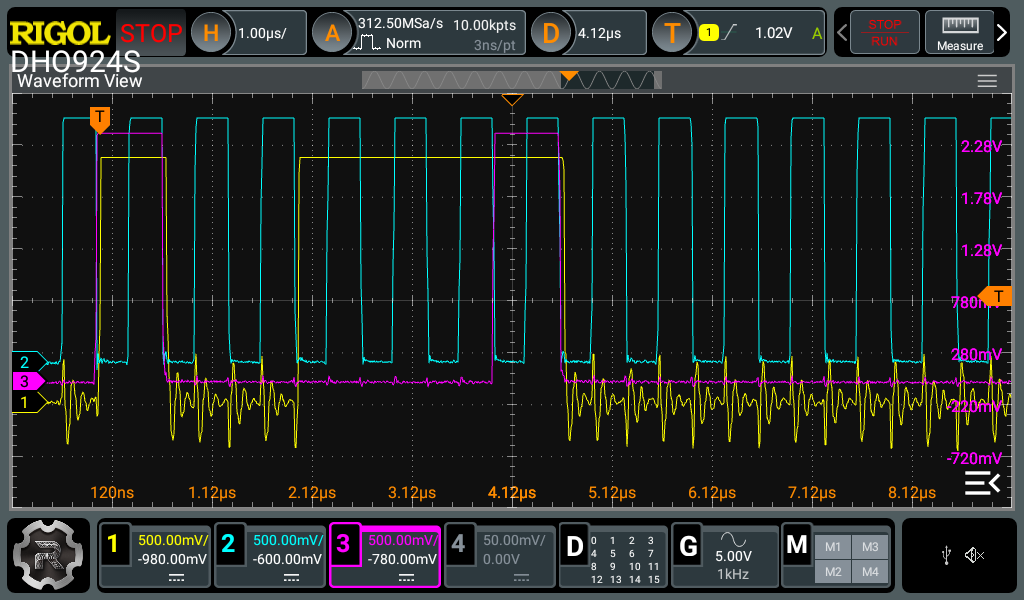
\includegraphics[width=\textwidth]{Pics/oszi_cube_spi_example.png}
	\caption{Screenshot des Osziloskopbildschirms. Dieser zeigt die Wellen für SCK (blau/türkis), MOSI (magenta) und MISO (gelb).}
	\label{fig:oszi_cube_spi_example}
\end{figure}



\begin{figure}[H]
	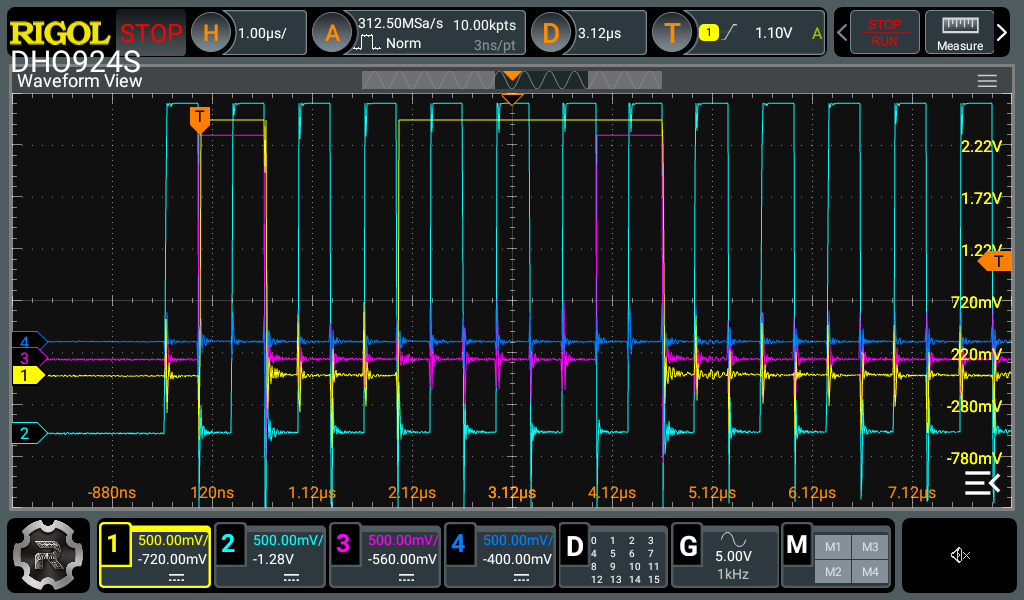
\includegraphics[width=\textwidth]{Pics/spi_signal_test.png}
	\caption{Screenshot einer erfolgreich SPI-Kommunikation, erstellt mit dem Code der HW\_API.}
	\label{fig:oszi_spi_signal_test}
\end{figure}


Die Testumgebung umfasste sowohl zwei Familien der STM32-Hardware (Nucleo-C031C6, Nucleo-G071RB, Nucleo-G0B1RE) als auch ein ESP32C6-DevKit, jeweils verbunden mit Debug-Schnittstellen und notwendiger Peripherie.
Die modulare Struktur, in der plattformspezifische Implementierungen klar gekapselt sind, ermöglicht neben der Übertragung der Lösung, auf unterschiedliche \gls{mcu}-Familien, ohne Anpassungen des Applikationscodes, auch die Erweiterung um fehlende Funktionsmodule oder neuer Microcontroller.
Einschränkungen bestehen lediglich in der begrenzten Testabdeckung, sowohl für STM32-Familien, als auch ESP32 Microcontroller, die nicht direkt validiert wurden.


\subsection{Weitere Erkenntnisse}
Im Zuge der Validierung der entwickelten HW\_API und deren Integration in bestehende HAL-Strukturen (STM32HAL, ESP32HAL) konnten neben den funktionalen Tests auch weitere technische Aspekte analysiert werden. 
Diese liefern zusätzliche Erkenntnisse über die Auswirkungen der neu eingeführten Abstraktionsschicht auf Codequalität, Performanz und Wartbarkeit.

\subsubsection{Buildgröße}
Um die Auswirkungen der Abstraktionsschicht \texttt{HW\_API} auf den Ressourcenverbrauch zu bewerten, wurden die Ausgaben am Ende des Buildprozesses mit einander verglichen.
In \cref{fig:stm32_cube_gpio_debug_size} präsentiert die Spalten Text, Data, Bss, Dec, Hex sowie den Dateinamen.
Die Spalte text repräsentiert den Programmspeicher (Flash), der neben dem  ausführbaren Code auch konstante Daten enthält. 
Die Spalten data und bss bilden auf den Arbeitsspeicher (RAM), wobei \textit{data} initialisierte globale und statische Variablen umfasst, die beim Start vom Flash in den RAM kopiert werden, während \textit{bss} uninitialisierte globale und statische Variablen beinhaltet, die beim Systemstart auf Null gesetzt werden. 
Die Spalten dec und hex repräsentieren die Gesamtspeicherbelegung in dezimaler bzw. hexadezimaler Form.
Das in VSCode erstellte Projekt, das die HW\_API mit verwendet, stellt die genannten Größen anders dar.
\cref{fig:stm32_hw_api_gpio_debug_size} zeigt die genutzte Größe (Used Size), die Gesamtgröße der Region (Region Size) und den prozentualen Anteil (\%age Used) für die Speicherbereiche RAM und Flash auf. 
Für die Analyse von Speicheränderungen ist die korrekte Zuordnung von Speicherbereichen von entscheidender Bedeutung. 
Die Flash-Belegung entspricht dabei der Text-Spalte, während die RAM-Belegung der Summe von data und bss entspricht; $RAM\ =\ data\ +\ bss$.


% stm32 cube debug
\begin{figure}[H]
	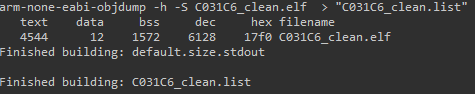
\includegraphics[width=\textwidth]{Pics/stm32c031c6_gpio_debug_size.png}
	\caption{Ausgabe des belegten Speichers in einem STM32CubeIDE Projekt.}
	\label{fig:stm32_cube_gpio_debug_size}
\end{figure}

% stm32 hw_api debug
\begin{figure}[H]
	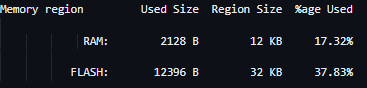
\includegraphics[width=\textwidth]{Pics/stm32c031c6_gpio_debug_size_hw_api.png}
	\caption{Ausgabe des belegten Speichers ein Projektes mit der HW\_API als zusätzliche Zwischenschicht.}
	\label{fig:stm32_hw_api_gpio_debug_size}
\end{figure}

Im Default-Build (\cref{fig:stm32_cube_gpio_debug_size}) zeigt die Speicherübersicht für das ELF-File C031C6\_clean.elf eine Flash-Belegung von $4\ 544$ Bytes (text) und eine RAM-Belegung von $1\ 584$ Bytes, die zusammengesetzt ist aus initialisierten (data, $12$ Bytes) und uninitialisierten (bss, $1\ 572$ Bytes) globalen bzw. statischen Variablen.

Dagegen zeigt das eigene Projekte mit der neuen HW\_API, eine Flash-Belegung von $12\ 396$ Bytes und eine RAM-Belegung von $2\ 128$ Bytes auf. Der Vergleich zeigt, dass die Einführung der Zwischenschicht zu einer Steigerung der Flash-Auslastung um $7\ 852$ Bytes und der RAM-Auslastung um $544$ Bytes geführt hat. 
Die Flash-Auslastung weist eine prozentuale Zunahme von etwa $14$\% auf knapp $38$\% auf, während die RAM-Auslastung von rund $13$\% auf $17$\% ansteigt.

Da es sich um Debug-Builds handelt, fallen die Binärgrößen aufgrund zusätzlicher Debug-Informationen größer aus als in optimierten Release-Builds und sind daher nicht direkt vergleichbar. 
Der Vergleich zeigt jedoch, dass die Einführung einer Zwischenschicht vor allem den Flash-Speicher deutlich stärker belastet, während die RAM-Nutzung nur moderat ansteigt. 
Dies veranschaulicht den signifikanten Einfluss zusätzlicher Abstraktionsschichten auf die Speicherressourcen und betont die Notwendigkeit einer sorgfältigen Planung hinsichtlich Flash- und RAM-Auslastung.

% esp sample
\begin{figure}[H]
	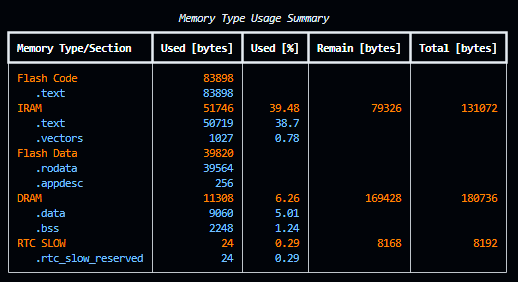
\includegraphics[width=\textwidth]{Pics/esp32c6_sample_project_size.png}
	\caption{Ausgabe des belegten Speichers eines Beispielprojekts mit der ESP-IDF.}
	\label{fig:esp32_sample_size}
\end{figure}

% esp hw_api
\begin{figure}[H]
	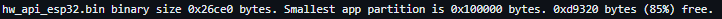
\includegraphics[width=\textwidth]{Pics/esp32c6_hw_api_debug_size.png}
	\caption{Ausgabe des belegten Speicher eines ESP32-Projektes mit der HW\_API-Zwischenschicht.}
	\label{fig:esp32_hw_api_size}
\end{figure}

Die Analyse der Speicherbelegung für den ESP32 zeigt, dass die Einführung einer zusätzlichen Zwischenschicht vor allem die Flash-Auslastung deutlich erhöht hat. 
Im Default-Build belegt das Programm $107\ 070$ Bytes Flash-Speicher, während das eigene Projekt mit Zwischenschicht eine Binärgröße von $158\ 944$ Bytes aufweist. 
Dies entspricht einer Zunahme von rund $51$ KB, also nahezu $48$\%. Unter Berücksichtigung einer verfügbaren App-Partition von $1$ MB ergibt sich eine Flash-Auslastung von ca. $15$\%, womit trotz des Anstiegs ausreichend Speicherreserven zur Verfügung stehen.

Die Bewertung der RAM-Auslastung anhand der kompakten Projektausgabe ist nicht direkt möglich, da diese lediglich die Flash-Größe ausweist. 
Die detaillierte ESP-IDF-Ausgabe des Default-Builds zeigt jedoch, dass neben Flash auch Bereiche wie DIRAM und LP SRAM genutzt werden. 
Um eine Aussage bezüglich potenzieller Modifikationen der RAM-Nutzung durch die Zwischenschicht treffen zu können, bedingt die Ausführung eines erweiterten Speicherreports, wie beispielsweise mittels \texttt{idf.py size --all}.


\subsubsection{Algorithmische Komplexität}
Die Analyse der GPIO-Klassen für STM32 und ESP32 ergibt, dass die algorithmische Komplexität aller Methoden konstant bleibt, d.h. $O(1)$. 
Die Tatsache, dass es sich in diesem Fall ausschließlich um Registerzugriffe oder Zustandsabfragen handelt, die unabhängig von der Anzahl der Pins oder der Systemgröße eine konstante Laufzeit aufweisen, ist für diese Beobachtung maßgeblich. 
Unterschiede ergeben sich lediglich in der Implementierung der Initialisierung.
Während beim STM32 ein Clock-Enable über eine switch-case-Struktur erforderlich ist, setzt der ESP32 direkt eine \texttt{gpio\_config\_t}-Struktur ein, in der die Pull-Widerstände ebenfalls über eine switch-case-Auswahl definiert werden. 
Diese Details haben jedoch keinen Einfluss auf die theoretische Laufzeitkomplexität.

Allerdings muss der Debounce-Funktionen eine besondere Aufmerksamkeit geschenkt werden muss. 
Sowohl auf STM32 als auch auf ESP32 sind sie als Zustandsautomaten mit mehreren Zuständen und Übergängen realisiert.
Obwohl die Komplexität auch hier konstant bleibt, resultiert die Vielzahl der Verzweigungen in einer höheren zyklomatischen Komplexität.

\subsubsection{Cyclomatic Complexity}
Die zyklomatische Komplexität (CC) stellt ein Maß für die Komplexität des Kontrollflusses innerhalb einer Methode oder Funktion dar. Sie gibt an, wie viele unabhängige Pfade durch den Code existieren. 

Die zyklomatische Komplexität kann gemäß der Formel nach McCabe $CC= E - N + 2P$ berechnet werden.
mit 
\begin{itemize}
	\item $E$ die Anzahl der Kanten (Verbindungen zwischen Anweisungen/Blöcken) im Kontrollflussgraphen ist,
	\item $N$ die Anzahl der Knoten (Anweisungen oder Blöcke) ist,
	\item $P$ die Anzahl der zusammenhängenden Komponenten (typischerweise 1 für eine einzelne Funktion) ist.
\end{itemize}

In beiden Plattformvarianten weisen die meisten Funktionen triviale Werte zwischen $1$ und $2$ auf, was eine hohe Lesbarkeit und Wartbarkeit begünstigt.

Im Fall von STM32 zeigt sich, dass die Funktion \texttt{port\_clock\_enable()} einen Ausreißer aufweist. 
Dieser ist auf die Realisierung der Auswahl des Ports über eine switch-case-Struktur mit mehreren Fällen zurückzuführen. 
Dies führt zu einer Erhöhung der CC auf Werte von $8$ bis $10$. 
Auch die Funktion \texttt{isDebouncePinOn()} weist durch ihre State-Machine eine erhöhte CC von etwa $8$ auf.

Die CC der Debounce-Funktion beträgt beim ESP32 ebenfalls in etwa $8$. 
Die Initialisierungsmethode \texttt{gpio\_init()} weist aufgrund der Konfiguration der Pull-Widerstände per Switch-Case eine etwas höhere CC auf.

Zusammenfassend lässt sich sagen, dass die Komplexität der GPIO-Implementierung insgesamt als überschaubar einzustufen ist. 
Die erhöhten Werte manifestieren sich ausschließlich in Funktionen, die dafür gedacht sind, eine Vielzahl von Zuständen abzudecken.).

\begin{table}[H]
\centering
	\begin{tabular}{@{}llp{4cm}p{2cm}p{2cm}@{}}
	\toprule
\textbf{Plattform} & \textbf{Methode} & \textbf{Beschreibung} & \textbf{Algorith. Komplex.} & \textbf{Cyclomatic Komplex.} \\ \midrule
STM32 & Konstruktor & Initialisierung der Member & O(1) & 1 \\
      & gpio\_init() & HAL-Struktur befüllen + Alternate & O(1) & 3 \\
      & readPin() & Direkter HAL-Aufruf & O(1) & 1 \\
      & writePin() & HAL-Aufruf mit Bedingung & O(1) & 2 \\
      & togglePin() & HAL-Aufruf zum Umschalten & O(1) & 1 \\
      & port\_clock\_enable() & Switch-case über Ports & O(1) & 8--10 \\
      & isPinOn() & Abfrage + Invertierung & O(1) & 2 \\
      & isDebouncePinOn() & Zustandsautomat, mehrere States & O(1) & 8 \\
      & Getter & Zugriff auf Member & O(1) & 1 \\ \midrule
ESP32 & Konstruktor & Initialisierung der Member & O(1) & 1 \\
      & gpio\_init() & gpio\_config\_t setzen + Pull via switch-case & O(1) & 5 \\
      & readPin() & Direkter HAL-Aufruf & O(1) & 1 \\
      & writePin() & Direkter HAL-Aufruf & O(1) & 1 \\
      & togglePin() & writePin(!readPin()) & O(1) & 1 \\
      & isPinOn() & Abfrage + Invertierung & O(1) & 2 \\
      & isDebouncePinOn() & Zustandsautomat mit 4 States & O(1) & 8 \\
      & Getter & Zugriff auf Member & O(1) & 1 \\ 
	\bottomrule
	\end{tabular}
	\caption{Algorithmische und zyklomatische Komplexität der GPIO-Klassen}
	\label{tab:gpio_complexity}
\end{table}


\subsubsection{Portabilität versus Optimierung}
Die Implementierung der Module mit einem objektorientierten Ansatz dient der Abstraktion der hardware-spezifischen Details über ein einheitliches Interface, wodurch identischer Anwendungscode sowohl auf STM32- als auch auf ESP32-Plattformen ausgeführt werden kann. 
Dieser Ansatz resultiert in einer signifikant erhöhten Portabilität, ist jedoch mit einem gewissen Overhead verbunden, da direkte Hardwarezugriffe über Hilfsfunktionen (z. B. modeToHAL(), pullToHAL()) geleitet werden. 

\subsubsection{Testbarkeit und Wartbarkeit}
Die klare Trennung von Schnittstellen und Implementierungen erleichtert die Modularisierung und damit die Durchführung von Unit Tests.
Die Kapselung der Pin-Initialisierung, Lese-/Schreiboperationen und Debouncing in klar abgegrenzte Methoden fördert die Testbarkeit. 
So kann jede Methode separat zu testen. 
Die Wartbarkeit wird durch konsistente Namenskonventionen und den modularen Aufbau des Systems zusätzlich unterstützt. 
Dadurch haben Änderungen an der Hardware-Abstraktion minimalen Einfluss auf die Anwendungsschicht.

\subsubsection{Kopplung und Abhängigkeiten}
Die Modulklasesn verwenden interne Hilfsfunktionen und Mappings der Enum-Classes, was eine geringen Kopplung an konkrete Hardwareregister zur Folge hat. 
Externe Abhängigkeiten beschränken sich auf HAL-Bibliotheken (STM32) oder ESP-IDF-Funktionen, wodurch der Rest des Codes unabhängig von der Plattform bleibt. 
Die Trennung von Interface und Implementierung reduziert die Kopplung weiter, sodass der Austausch einer Plattformimplementierung nur minimale Änderungen erfordert.

\subsubsection{Codequalität}
Die Klassen weisen durchgängig einen modernen, lesbaren C++-Stil auf, der durch klare Initialisierung, Nutzung von \texttt{enum class}, \texttt{[[nodiscard]]}-Attributen und \texttt{assert}-basierten Sicherheitsprüfungen gekennzeichnet ist. 
Zyklomatische und algorithmische Komplexität bleiben in einem überschaubaren Bereich, was die Verständlichkeit und Wartbarkeit des Systems unterstützt.
Weiterhin besteht die Möglichkeit, die Performance durch potenzielle Optimierungen, wie die Reduzierung von Switch-Statements oder Inline-Funktionen, leicht zu erhöhen.

\subsubsection{Integration in Buildsysteme}
Die Trennung von plattformunabhängiger HW\_API und plattformspezifischer Implementierung erleichtert die Integration in unterschiedliche Buildsysteme wie STM32CubeIDE oder ESP-IDF. 
Die Struktur verwendet bereits mit \texttt{\#ifdef} bedingte Kompilierung, sodass je nach Zielplattform die korrekte Implementierung kompiliert wird, ohne dass eine Anpassung des Anwendungscodes erforderlich ist. 
Dies gewährleistet reproduzierbare Builds und reduziert das Risiko von Konfigurationsfehlern.

\vspace{1cm}
Zusammenfassend lässt sich festhalten, dass die Einführung der HW\_API nicht nur funktionale Vorteile in Bezug auf die Portabilität bietet, sondern auch Auswirkungen auf Ressourcenverbrauch, Komplexität und Wartbarkeit hat. 
Diese müssen in der Embedded-Entwicklung stets berücksichtigt und gegeneinander abgewogen werden. 
Die Validierung hat ergeben, dass die HW\_API die geforderten funktionalen Anforderungen erfüllt, korrekt arbeitet und somit eine stabile Grundlage für die Implementierung plattformunabhängiger Embedded-Anwendungen darstellt. 
Die gewählten Testmethoden ermöglichten zudem eine nachvollziehbare und reproduzierbare Überprüfung der Softwarequalität.






























